% !TeX spellcheck = <none>
\documentclass[a4paper,12pt,onecolumn,oneside]{article}
\usepackage{cite} % bibTeX引用
\usepackage[UTF8]{ctex}
\usepackage{booktabs}
\usepackage{graphicx} % 用于插入图片
\usepackage{amsmath} % 数学公式
\usepackage{hyperref} % 超链接
\usepackage{caption} % 图片标题
\usepackage{subcaption} % 子图片
\usepackage{geometry}
\geometry{a4paper,scale=0.8}

\usepackage{titlesec}
\titleformat{\section}
{\normalfont\Large\bfseries\centering}{\thesection}{1em}{}

\usepackage{subcaption}
\usepackage[table]{xcolor}
\usepackage{colortbl}
\usepackage{listings}

\lstset{
	numbers=left, %设置行号位置
	numberstyle=\tiny, %设置行号大小
	keywordstyle=\color{blue}, %设置关键字颜色
	commentstyle=\color[cmyk]{1,0,1,0}, %设置注释颜色
	frame=single, %设置边框格式
	escapeinside=``, %逃逸字符(1左面的键),用于显示中文
	%breaklines, %自动折行
	extendedchars=false, %解决代码跨页时,章节标题,页眉等汉字不显示的问题
	xleftmargin=2em,xrightmargin=2em, aboveskip=1em, %设置边距
	tabsize=4, %设置tab空格数
	showspaces=false %不显示空格
}


\title{二手帆船价格数据集上的k-NN回归建模}
\author{第十组}
\date{\today}

\begin{document}
	\maketitle
	
\begin{abstract}
	当前,使用k-NN回归算法进行建模已经成为数据科学领域中一个广泛应用的技术。本文利用k-NN回归算法对二手帆船价格数据进行建模,并比较了使用曼哈顿距离、马哈拉诺比斯距离、欧几里得距离进行回归分析的效果。同时,本文还逐步删去了几个变量重新建模,并得到了几个比较好的模型,并和广义回归模型进行比较。本文的研究结果为二手帆船市场的价格预测提供了新的方法和思路,对于该领域的研究和实践具有一定的参考价值。
\end{abstract}

	\tableofcontents
	\clearpage
	\section{k-NN回归算法介绍}
	
	\subsection{算法原理}
	k-最近邻算法,也称k-NN算法,是一种非参数、有监督的学习分类器,它使用邻近度对单个数据点的分组进行分类或预测。虽然k-NN算法最常被用于离散值的分类问题,但它也可用于连续值的回归问题。具体来说,k-NN回归算法的原理可以概括为以下几个步骤:
	\begin{enumerate}
		\item 选择一个适当的k值,表示在训练集中选择k个最近邻居作为预测新数据点的参考。
		\item 对于给定的新数据点,计算它与所有训练数据点之间的距离,并选择k个距离最近的训练数据点作为预测的邻居。
		\item 将这k个邻居的数值输出取平均值,作为新数据点的预测输出值。
	\end{enumerate}
	在实现k-NN算法之前,我们需要首先定义距离。接下来介绍几种我们建模过程中使用的距离定义。
	
	\subsection{几种k-NN算法常用的距离}
	\paragraph{欧几里得距离} 欧几里得距离是最常用的距离度量,指在$n$维空间中两个点之间的真实距离,仅限于实值向量。$x$与$y$之间的欧氏距离由以下公式定义:
	\begin{equation*}
		Euclidean~distance = d(x,y) = \sqrt{\sum_{i=1}^{n}(y_i-x_i)^2}
	\end{equation*}
	\paragraph{曼哈顿距离} 曼哈顿距离指的是在$n$维欧几里得空间的固定直角坐标系上,两点所形成的线段对轴产生的投影的距离总和,其定义为:
	\begin{equation*}
		Manhattan~distance = d(x,y) = \sum_{i=1}^{n}|x_i-y_i|
	\end{equation*}
	\paragraph{马哈拉诺比斯距离} 马哈拉诺比斯距离是由印度统计学家普拉桑塔·钱德拉·马哈拉诺比斯提出的一种基于样本分布的距离定义,表示数据的协方差距离。相比于欧氏距离,它消除了量纲对距离的影响。假设$x, y$是从均值向量为$\mu$,协方差矩阵为$\Sigma$的总体$\Omega$中随机抽取的两个样本,定义$x, y$两点之间的马氏距离为
	\begin{equation*}
		Mahalanobis~distance = d^{2}(x,y) = (x-y)^{\top}\Sigma^{-1}(x-y)
	\end{equation*}
	定义$x$与总体$\Omega$的马氏距离为
	\begin{equation*}
		d^{2}(x,\mu_{\Omega}) = (x-\mu_{\Omega})^{\top}\Sigma^{-1}(x-\mu_{\Omega})
	\end{equation*}
	
	\section{数据集}  % 介绍你使用的二手帆船价格数据集,包括数据集的属性、大小、格式等。
	通过爬虫技术得到了二手帆船价格及其影响因素的1174条数据,含有10个自变量。数据说明如表\ref{tab:boat-variables}。\par 
	
	\begin{table}[h]
		\centering
		\caption{帆船数据变量}
		\vspace{0.25\baselineskip}
		\label{tab:boat-variables}
		\begin{tabular}{cccc}
			\toprule
			变量名 & 变量类型 & 取值范围 & 备注 \\ \midrule
			ID & —— & Eg.Boat0001 & 帆船编号 \\ 
			Year & 连续型(自变量$x_1$) & [2005,2019] & 帆船出厂年份 \\ 
			Length & 连续型(自变量$x_2$) & [37.5,56] & 帆船长度 \\ 
			LWL & 连续型(自变量$x_3$) & [36.08,56.08] & 帆船设计水线长 \\ 
			Beam & 连续型(自变量$x_4$) & [19.67,24.21] & 帆船船宽 \\ 
			Draft & 连续型(自变量$x_5$) & [2.92,6.92] & 帆船吃水深度 \\ 
			Displacement & 连续型(自变量$x_6$) & [11000,77162] & 帆船排水量 \\ 
			SailArea & 连续型(自变量$x_7$) & [753,2626] & 帆船帆面积 \\ 
			GDP & 连续型(自变量$x_8$) & [0.6,3861] & 售卖地区的国内生产总值 \\ 
			GDP.Capita & 连续型(自变量$x_9$) & [2222,93667] & 售卖地区的人均国内生产总值 \\ \hline
			Price & 连续型(因变量$y$) & [95000,2890000] & 帆船的挂牌价格 \\ \bottomrule
		\end{tabular}
	\end{table}
	
	\section{模型建立}  % 描述你的实验,包括数据预处理、特征工程、模型训练和评估等。
	\subsection{数据预处理}  % 描述你的数据预处理过程,包括缺失值处理、异常值处理等。
	由于自变量ID(帆船编号)对建模无帮助,故删除。选取剩余数据作为特征变量,对价格(Price)变量进行异常值处理。使用boxplot函数对价格这个变量进行可视化,然后得到该变量的下限和上限。接着使用这个下限和上限对价格进行过滤,保留价格在该范围内的数据。具体实现见Listing \ref{lst:1}.
	\begin{lstlisting}[language=R, caption={异常值处理}, label={lst:1},belowcaptionskip=0.5\baselineskip]
price = read.csv("Boats.csv",fileEncoding = 'gbk',header=T)
price = price[c(1:961),c(2:11)]  # 删掉第一列
pic = boxplot(price$Price)
low = pic$stats[1]
up = pic$stats[5]
price = price[price$Price>=low&price$Price<=up,]
str(price)
	\end{lstlisting}  
	\subsection{准备工作}
	此后,我们计算特征变量之间的相关性,然后使用corrplot函数绘制相关矩阵的可视化图形,如图\ref{fig:corrplot}所示。\par 
	\begin{figure}[h]
		\centering
		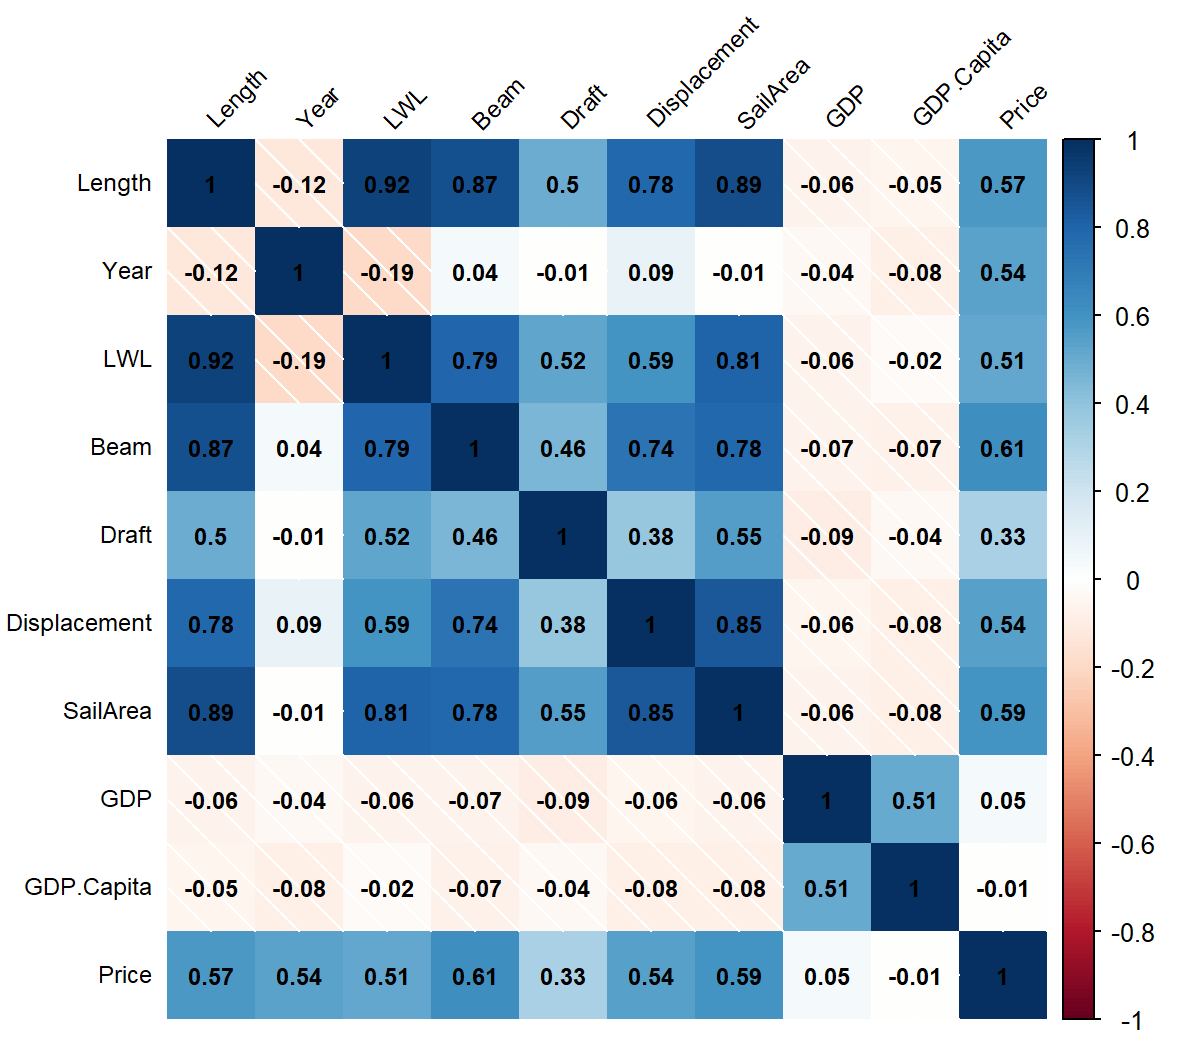
\includegraphics[width=\textwidth]{res/corrplot.png}
		\caption{相关矩阵热力图}
		\label{fig:corrplot}
	\end{figure}
	通过观察图像,发现GDP.Capita和GDP两个变量与因变量关系小,在后续的工作中,我们可以考虑删除这两个变量。接下来,使用sample函数将数据集按照7:3划分为训练集和测试集。最后,使用caret库中的trainControl函数,选择10折交叉验证方法,然后使用expand.grid函数选取2到10不同的K值,用于后续的网格搜索。
	
	\begin{lstlisting}[language=R, caption={准备工作}, label={lst:2},belowcaptionskip=0.5\baselineskip]
library(corrplot)
corr=cor(price)
corrplot(corr, method = 'shade', type = "full",
addCoef.col = "black", number.cex = 0.75,
tl.cex = 0.75, tl.col = "black", tl.srt = 45)
set.seed(20)
train=sample(1:926,648) 
train_price=price[train,]
test_price=price[-train,]
library(caret)
control <- trainControl(method = 'cv',number = 10)
k_values <- data.frame(k = 2:10)
grid <- expand.grid(.k = k_values)
	\end{lstlisting}
	\subsection{模型训练}  % 描述你的模型训练过程,包括模型的选择、参数的选择等。
	\subsubsection{基于曼哈顿距离的回归模型}

	\paragraph{model11}如\ref{lst:3}所示,首先对自变量进行中心化和标准化处理,以消除量纲。接下来,设置交叉验证方法为10折交叉验证,将k值从2到10进行网格搜索寻找最佳的k值。用训练好的模型对测试集进行预测,并将预测结果存储在结果变量中。得到模型model11如表\ref{tbl:model11}所示,其中,性能指标包括均方根误差(RMSE)、决定系数(R$^2$)和平均绝对误差(MAE)。\par 
	通过比较不同的k值,发现k=3时,模型具有最小的RMSE和最高的R$^2$。在这个k值下,模型的RMSE为65222.08,即预测值与真实值的平均偏差为65222.08美元,而MAE为46993.80,即预测值与真实值的平均绝对偏差为46993.80美元,对于平均价格为43万元左右的二手帆船来说,这个偏差值不算大;模型的R$^2$为0.7630458,即模型能够解释目标变量变异的76.51$\%$,表明模型对帆船价格的预测比较准确。
\begin{lstlisting}[language=R, caption={knn回归,曼哈顿距离}, label={lst:3}, belowcaptionskip=0.5\baselineskip]
set.seed(20)
model11 <- train(Price~.,train_price,  # 用训练集进行模型训练
		   method = 'knn',
		   preProcess = c('center','scale'),  # 对自变量进行中心化与标准化以消除量纲
           trControl = control,
           tuneGrid = grid, distance = "manhattan")  # 选取距离度量为曼哈顿距离
model11   #查看模型效果
predict11=predict(model11,newdata=test_price)  # 将模型应用于测试集进行预测
\end{lstlisting}
	\paragraph{model12}在前一模型的基础上,删除自变量中的Draft变量,重新进行训练得到模型model12,其性能指标如表\ref{tbl:model12}所示。当k=6时,模型效果最好。
	\paragraph{model13}在前一模型的基础上,删除自变量中的GPD.Capita变量,重新进行训练得到模型model13,其性能指标如表\ref{tbl:model13}所示。当k=5时,模型效果最好。
	\paragraph{model14}最后再删除自变量中的Length变量,重新进行训练得到模型model14,其性能指标如表\ref{tbl:model14}所示。当k=5时模型效果最好。\par 
	将曼哈顿距离的knn算法模型预测结果与测试集中的真实价格值放入向量x中,并按照真实值由小到大排序。绘制x中的真实值与预测值效果图进行效果查看,对比测试集真值、9、8、7、6维度(分别对应model11-model14)的模型预测结果,如图\ref{fig:manhattan}所示。
	\vspace{\baselineskip}	
	\begin{table}[h]
		\centering
		\begin{subtable}{0.45\textwidth}
			\centering
				\begin{tabular}{cccc}
			\toprule
			k & RMSE & R$^2$ & MAE \\
			\midrule
			2 & 67887.72 & 0.7422961 & 48704.81 \\
			\rowcolor{gray!25}3 & 65222.08 & 0.7630458 & 46993.80 \\
			4 & 66316.32 & 0.7515969 & 48363.23 \\
			5 & 65747.23 & 0.7562927 & 48532.32 \\
			6 & 66125.31 & 0.7526372 & 49078.03 \\
			7 & 65342.83 & 0.7579675 & 48538.83 \\
			8 & 66668.73 & 0.7480789 & 49503.23 \\
			9 & 67512.24 & 0.7413292 & 50274.44 \\
			10 & 68334.18 & 0.7352037 & 51042.36 \\
			\bottomrule
		\end{tabular}
		\caption{model11的不同$k$值下的性能指标}
		\label{tbl:model11}
		\end{subtable}
		\hfill
		\begin{subtable}{0.45\textwidth}
			\centering
		\begin{tabular}{cccc}
		\toprule
		k & RMSE & R$^2$ & MAE \\
		\midrule
		2 & 67498.95 & 0.7425401 & 48696.57 \\
		3 & 66628.95 & 0.7489858 & 48208.85 \\
		4 & 65848.06 & 0.7558077 & 47964.54 \\
		5 & 64581.26 & 0.7650610 & 47710.74 \\
		\rowcolor{gray!25}6 & 64434.59 & 0.7646532 & 48322.29 \\
		7 & 64623.12 & 0.7633599 & 48401.10 \\
		8 & 65674.85 & 0.7557588 & 49165.32 \\
		9 & 66373.03 & 0.7516587 & 49856.13 \\
		10 & 67043.64 & 0.7473225 & 50477.92 \\
		\bottomrule
		\end{tabular}
		\caption{model12的不同$k$值下的性能指标}
		\label{tbl:model12}
		\end{subtable}
	\end{table}
	\begin{table}
		\begin{subtable}{0.45\textwidth}
			\centering
			\begin{tabular}{cccc}
				\toprule
				k & RMSE & R$^2$ & MAE \\
				\midrule
				2 & 65740.98 & 0.7578868 & 47484.90 \\
				3 & 64313.55 & 0.7658585 & 45944.23 \\
				4 & 63749.53 & 0.7685846 & 45583.04 \\
				\rowcolor{gray!25}5 & 63184.94 & 0.7714663 & 45809.52 \\
				6 & 63362.28 & 0.7697086 & 46302.68 \\
				7 & 64021.72 & 0.7648071 & 46987.42 \\
				8 & 65051.79 & 0.7585085 & 48004.02 \\
				9 & 65459.41 & 0.7565962 & 48465.62 \\
				10 & 66346.20 & 0.7492986 & 49125.57 \\
				\bottomrule
			\end{tabular}
			\caption{model13的不同$k$值下的性能指标}
			\label{tbl:model13}
		\end{subtable}
		\hfill
		\begin{subtable}{0.45\textwidth}
			\centering
				\begin{tabular}{cccc}
				\toprule
				k & RMSE & R$^2$ & MAE \\
				\midrule
				2 & 66860.03 & 0.7492369 & 47814.90\\
				3 & 65526.00 & 0.7572881 & 46733.80\\
				4 & 64727.59 & 0.7615374 & 45808.72\\
				\rowcolor{gray!25}5 & 63947.72 & 0.7658753 & 46324.00\\
				6 & 64380.97 & 0.7619273 & 46961.27\\
				7 & 64823.59 & 0.7588512 & 47864.96\\
				8 & 65379.83 & 0.7562327 & 48675.71\\
				9 & 65506.10 & 0.7566043 & 48837.97\\
				10 & 66374.46 & 0.7488659 & 49490.68\\
				\bottomrule
			\end{tabular}
			\caption{model14的不同$k$值下的性能指标}
			\label{tbl:model14}
		\end{subtable}
	\end{table}
	\begin{figure}[h]
		\centering
		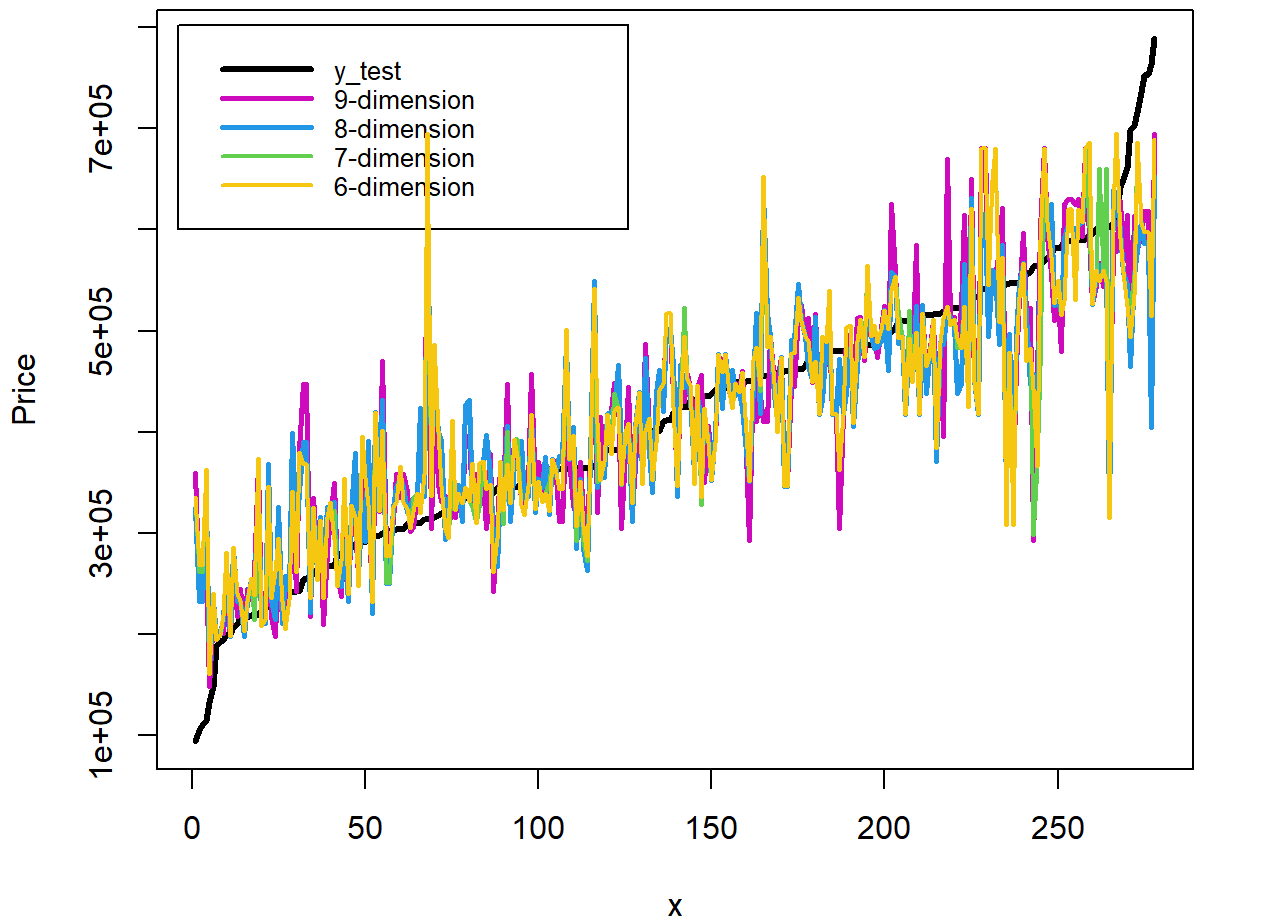
\includegraphics[width=0.73\textwidth]{res/manhattan.png}
		\caption{曼哈顿距离模型效果图}
		\label{fig:manhattan}
	\end{figure}
	\clearpage
	\subsubsection{基于马氏距离的回归模型}
	\paragraph{model21}类似于训练曼哈顿距离定义下的模型,我们先不去除任何变量训练获得模型model21,其性能指标如表\ref{tbl:model21}所示。当k=5时,模型效果最好。
\begin{lstlisting}[language=R, caption={knn回归,马氏距离}, label={lst:4}, belowcaptionskip=0.5\baselineskip]
set.seed(20)
model21 <- train(Price~.,train_price,
method = 'knn',
preProcess = c('center','scale'),
trControl = control,
tuneGrid = grid, distance = "mahalanobis", mahal = mahal)
model21  # 查看模型效果(自变量全保留)
predict21=predict(model21,newdata=test_price)  # 将模型应用于测试集进行预测
\end{lstlisting}
	\paragraph{model22}去除变量Beam,获得模型model22,如表\ref{tbl:model22}所示。当k=3时,模型效果最好。
	\paragraph{model23}再去除变量GDP.Capita得模型model23,如表\ref{tbl:model23}所示。当k=4时,模型效果最好。
	\paragraph{model24}最后去除变量Draft得模型model24,如表\ref{tbl:model24}所示。当k=5时,模型效果最好。\par
		\begin{table}[h]
		\centering
		\begin{subtable}{0.45\textwidth}
			\centering
			\begin{tabular}{cccc}
				\toprule
				k & RMSE & R$^2$ & MAE \\
				\midrule
				2 & 66860.03 & 0.7492369 & 47814.90\\
				3 & 65526.00 & 0.7572881 & 46733.80\\
				4 & 64727.59 & 0.7615374 & 45808.72\\
\rowcolor{gray!25}5 & 63947.72 & 0.7658753 & 46324.00\\
				6 & 64380.97 & 0.7619273 & 46961.27\\
				7 & 64823.59 & 0.7588512 & 47864.96\\
				8 & 65379.83 & 0.7562327 & 48675.71\\
				9 & 65506.10 & 0.7566043 & 48837.97\\
				10 & 66374.46 & 0.7488659 & 49490.68\\
				\bottomrule
			\end{tabular}
			\caption{model21的不同$k$值下的性能指标}
			\label{tbl:model21}
		\end{subtable}
		\hfill
		\begin{subtable}{0.45\textwidth}
			\centering
			\begin{tabular}{cccc}
				\toprule
				k & RMSE & R$^2$ & MAE \\
				\midrule
				2 & 66329.90 & 0.7520185 & 47439.89\\
\rowcolor{gray!25}3 & 64301.94 & 0.7699990 & 46360.91\\
				4 & 65189.65 & 0.7611171 & 47460.44\\
				5 & 65995.04 & 0.7541043 & 48200.98\\
				6 & 66882.32 & 0.7469734 & 49159.63\\
				7 & 66596.40 & 0.7479714 & 49044.68\\
				8 & 67500.67 & 0.7411828 & 49875.66\\
				9 & 67780.76 & 0.7392789 & 50316.05\\
				10 & 69076.04 & 0.7301169 & 51023.09\\
				\bottomrule
			\end{tabular}
			\caption{model22的不同$k$值下的性能指标}
			\label{tbl:model22}
		\end{subtable}
		\end{table}
		\begin{table}
		\begin{subtable}{0.45\textwidth}
			\centering
			\begin{tabular}{cccc}
				\toprule
				k & RMSE & R$^2$ & MAE \\
				\midrule
				2 & 65637.11 & 0.7574311 & 47597.82\\
				3 & 64691.20 & 0.7668326 & 46409.13\\
\rowcolor{gray!25}4 & 64036.75 & 0.7668532 & 45408.26\\
				5 & 64500.84 & 0.7623201 & 46171.07\\
				6 & 64535.21 & 0.7623190 & 46386.54\\
				7 & 64922.46 & 0.7601220 & 46786.40\\
				8 & 65293.03 & 0.7585225 & 47801.88\\
				9 & 65426.86 & 0.7577260 & 48030.91\\
				10 & 66225.62 & 0.7518083 & 48858.24\\
				\bottomrule
			\end{tabular}
			\caption{model23的不同$k$值下的性能指标}
			\label{tbl:model23}
		\end{subtable}
		\hfill
		\begin{subtable}{0.45\textwidth}
			\centering
			\begin{tabular}{cccc}
				\toprule
				k & RMSE & R$^2$ & MAE \\
				\midrule
				2 & 64527.59 & 0.7652540 & 46803.09\\
				3 & 62938.60 & 0.7762273 & 45409.70\\
				4 & 62369.63 & 0.7790298 & 44522.20\\
\rowcolor{gray!25}5 & 61675.29 & 0.7826572 & 44665.89\\
				6 & 62490.90 & 0.7760066 & 45517.03\\
				7 & 63468.60 & 0.7696194 & 46577.33\\
				8 & 64395.55 & 0.7637989 & 47633.79\\
				9 & 64788.57 & 0.7622317 & 48147.95\\
				10 & 65132.30 & 0.7600609 & 48556.00\\
				\bottomrule
			\end{tabular}
			\caption{model24的不同$k$值下的性能指标}
			\label{tbl:model24}
		\end{subtable}
	\end{table}
	将马氏距离的knn算法模型预测结果与测试集中的真实价格值放入向量y中,并按照真实值由小到大排序。绘制y中的真实值与预测值效果图进行效果查看,对比测试集真值、9、8、7、6维度(分别对应model21-model24)的模型预测结果,如图\ref{fig:mashi}所示。
	\vspace{\baselineskip}
	\begin{figure}[h]
	\centering
	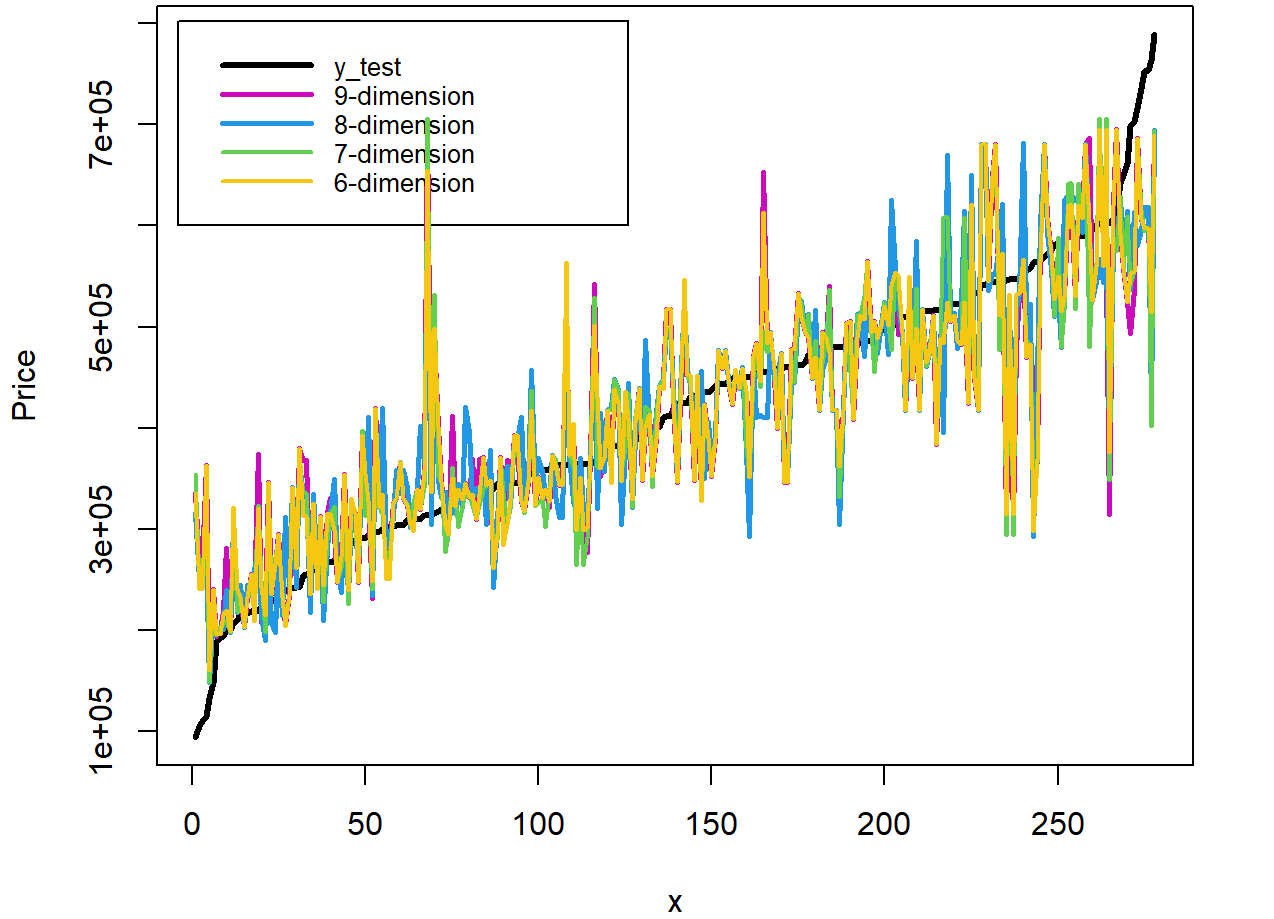
\includegraphics[width=0.73\textwidth]{res/mashi.png}
	\caption{马氏距离模型效果图}
	\label{fig:mashi}
	\end{figure}
	\clearpage
	\subsubsection{基于欧氏距离的回归模型}
	\paragraph{model31}类似于训练曼哈顿距离定义下的模型,我们先不去除任何变量训练获得模型model21,其性能指标如表\ref{tbl:model21}所示。当k=5时,模型效果最好。
\begin{lstlisting}[language=R, caption={knn回归,欧氏距离}, label={lst:5}, belowcaptionskip=0.5\baselineskip]
set.seed(20)
model31 <- train(Price~.,train_price,
method = 'knn',
preProcess = c('center','scale'),
trControl = control,
tuneGrid = grid, distance = "euclidean")
model31 #查看模型效果(自变量全保留)
predict31=predict(model31,newdata=test_price)#将模型应用于测试集进行预测
\end{lstlisting}
	\paragraph{model32}去除变量Beam,获得模型model22,如表\ref{tbl:model22}所示。当k=3时,模型效果最好。
	\paragraph{model33}再去除变量GDP.Capita得模型model23,如表\ref{tbl:model23}所示。当k=4时,模型效果最好。
	\paragraph{model34}最后去除变量Draft得模型model24,如表\ref{tbl:model24}所示。当k=5时,模型效果最好。
	
	\begin{table}[h]
	\centering
	\begin{subtable}{0.45\textwidth}
		\centering
		\begin{tabular}{cccc}
			\toprule
			k & RMSE & R$^2$ & MAE \\
			\midrule
		2 & 64527.59 & 0.7652540 & 46803.09\\
		3 & 62938.60 & 0.7762273 & 45409.70\\
		4 & 62369.63 & 0.7790298 & 44522.20\\
\rowcolor{gray!25}5 & 61675.29 & 0.7826572 & 44665.89\\
		6 & 62490.90 & 0.7760066 & 45517.03\\
		7 & 63468.60 & 0.7696194 & 46577.33\\
		8 & 64395.55 & 0.7637989 & 47633.79\\
		9 & 64788.57 & 0.7622317 & 48147.95\\
		10 & 65132.30 & 0.7600609 & 48556.00\\
			\bottomrule
		\end{tabular}
		\caption{model31的不同$k$值下的性能指标}
		\label{tbl:model31}
	\end{subtable}
	\hfill
	\begin{subtable}{0.45\textwidth}
		\centering
		\begin{tabular}{cccc}
			\toprule
			k & RMSE & R$^2$ & MAE \\
			\midrule
			2 & 66329.90 & 0.7520185 & 47439.89\\
\rowcolor{gray!25}3 & 64301.94 & 0.7699990 & 46360.91\\
			4 & 65189.65 & 0.7611171 & 47460.44\\
			5 & 65995.04 & 0.7541043 & 48200.98\\
			6 & 66882.32 & 0.7469734 & 49159.63\\
			7 & 66596.40 & 0.7479714 & 49044.68\\
			8 & 67500.67 & 0.7411828 & 49875.66\\
			9 & 67780.76 & 0.7392789 & 50316.05\\
			10 & 69076.04 & 0.7301169 & 51023.09\\
			\bottomrule
		\end{tabular}
		\caption{model32的不同$k$值下的性能指标}
		\label{tbl:model32}
	\end{subtable}
	\end{table}
	\begin{table}
	\begin{subtable}{0.45\textwidth}
		\centering
		\begin{tabular}{cccc}
			\toprule
			k & RMSE & R$^2$ & MAE \\
			\midrule
			2 & 65928.85 & 0.7551167 & 47230.63\\
			3 & 63712.48 & 0.7723549 & 46424.42\\
			4 & 64635.72 & 0.7636695 & 47132.27\\
\rowcolor{gray!25}5 & 63029.12 & 0.7757735 & 46704.58\\
			6 & 63536.83 & 0.7717490 & 47561.70\\
			7 & 64165.60 & 0.7678010 & 47847.44\\
			8 & 65725.69 & 0.7555275 & 48824.82\\
			9 & 66881.12 & 0.7490636 & 50062.24\\
			10 & 66922.39 & 0.7494815 & 50229.53\\
			\bottomrule
		\end{tabular}
		\caption{model33的不同$k$值下的性能指标}
		\label{tbl:model33}
	\end{subtable}
	\hfill
	\begin{subtable}{0.45\textwidth}
		\centering
		\begin{tabular}{cccc}
			\toprule
			k & RMSE & R$^2$ & MAE \\
			\midrule
			2 & 64527.59 & 0.7652540 & 46803.09\\
			3 & 62938.60 & 0.7762273 & 45409.70\\
			4 & 62369.63 & 0.7790298 & 44522.20\\
\rowcolor{gray!25}5 & 61675.29 & 0.7826572 & 44665.89\\
			6 & 62490.90 & 0.7760066 & 45517.03\\
			7 & 63468.60 & 0.7696194 & 46577.33\\
			8 & 64395.55 & 0.7637989 & 47633.79\\
			9 & 64788.57 & 0.7622317 & 48147.95\\
			10 & 65132.30 & 0.7600609 & 48556.00\\
			\bottomrule
		\end{tabular}
		\caption{model34的不同$k$值下的性能指标}
		\label{tbl:model34}
	\end{subtable}
\end{table}
	将欧氏距离的knn算法模型预测结果与测试集中的真实价格值放入向量z中,并按照真实值由小到大排序。绘制z中的真实值与预测值效果图进行效果查看,对比测试集真值、9、8、7、6维度(分别对应model31-model34)的模型预测结果,如图\ref{fig:eucilid}所示。
	\begin{figure}[h]
	\centering
	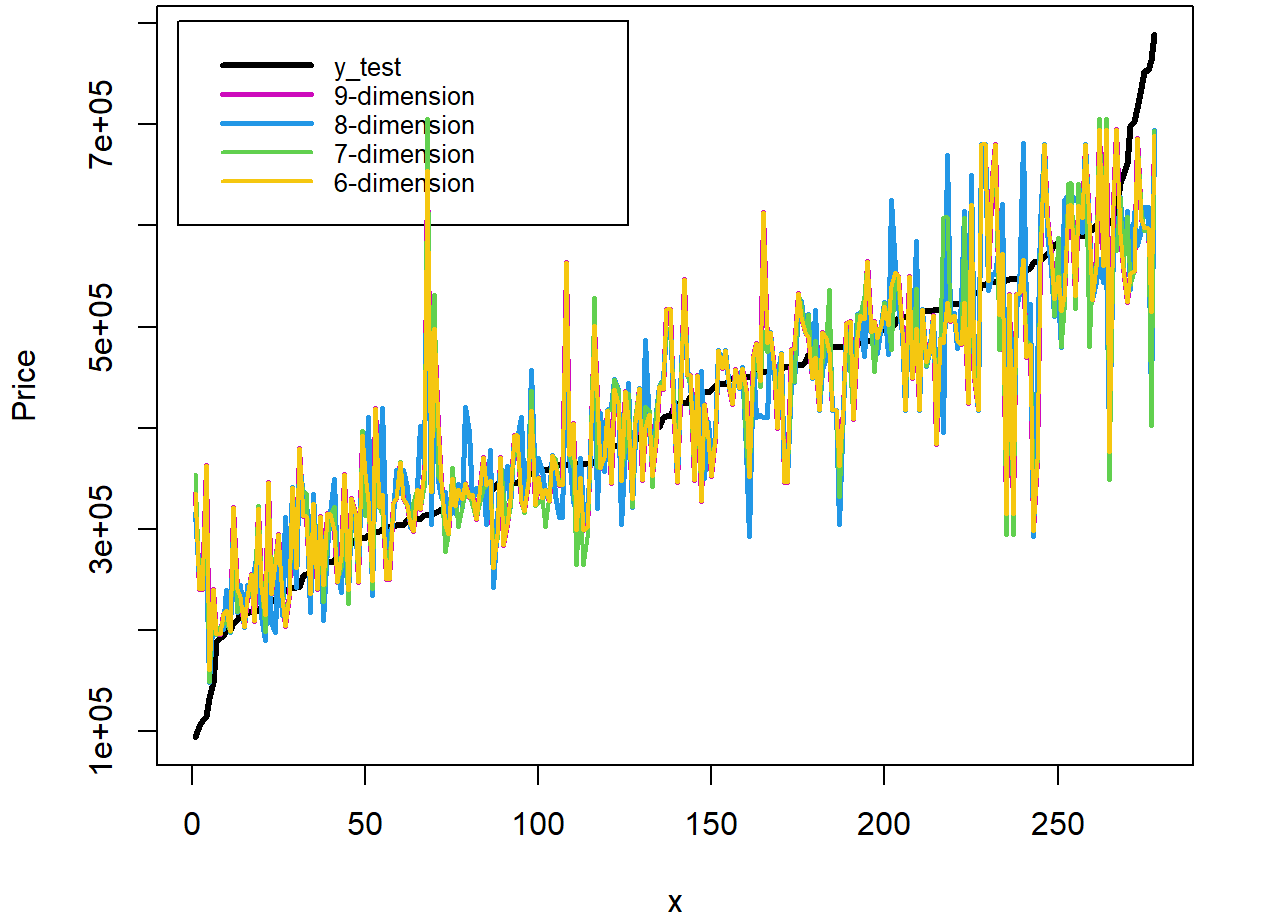
\includegraphics[width=0.73\textwidth]{res/eucilid.png}
	\caption{欧氏距离模型效果图}
	\label{fig:eucilid}
	\end{figure}
	
	\subsection{模型评估}
	经过对比,我们发现模型model11, model31, model34, model24的效果较好。为了进一步评估k-NN回归的效果,将这四个模型与线性回归模型中的广义线性回归模型进行对比。在我们先前的工作中,广义回归模型是三种线性回归模型中表现最好的。比较五个模型预测值与真实值的对比如图\ref{fig:duibi}所示。\par
	\begin{figure}[h]
	\centering
	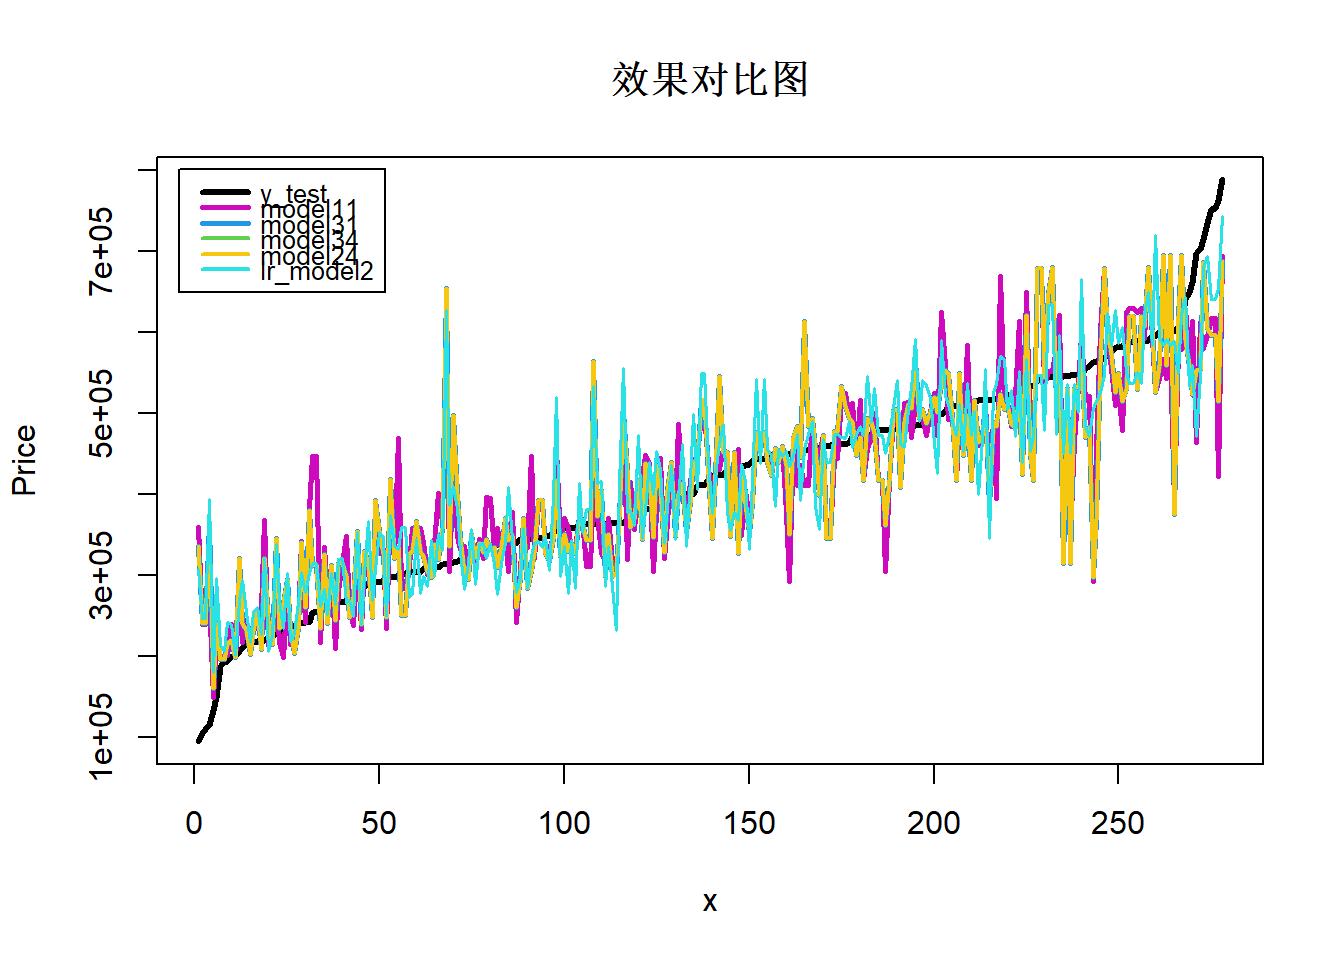
\includegraphics[width=\textwidth]{res/duibi.png}
	\caption{model11, 31, 34, 24与广义线性回归效果对比图}
	\label{fig:duibi}
	\end{figure}
	根据图片直观显示,广义回归模型的预测效果仍旧是比较好的。进一步地,我们可以比较每个k-NN回归模型在最佳k值下的$R^2$和广义回归模型的$R^2$,发现广义回归模型的$R^2$为0.7958,而k-NN模型最佳的$R^2$是0.7826. 因此,我们认为k-NN回归模型相较于广义回归模型在预测二手帆船价格方面并没有突出的优势。
	\section{总结}
	针对二手帆船价格数据集,我们分别建立了基于曼哈顿距离、马哈拉诺比斯距离和欧几里得距离的k-NN回归模型,并对模型的预测效果进行了评价。将效果最好的模型与先前工作中已证实效果较好的广义回归模型进行对比,发现k-NN回归模型在预测效果上不如广义回归模型,这说明数据集并不非常适合使用k-NN回归模型进行建模。
\end{document}
